\documentclass[12pt]{article}

\usepackage{amsmath, mathtools}
\usepackage{amsfonts}
\usepackage{amssymb}
\usepackage{graphicx}
\usepackage{colortbl}
\usepackage{xr}
\usepackage{hyperref}
\usepackage{longtable}
\usepackage{xfrac}
\usepackage{tabularx}
\usepackage{float}
\usepackage{siunitx}
\usepackage{booktabs}
\usepackage{caption}
\usepackage{pdflscape}
\usepackage{afterpage}

\usepackage[round]{natbib}

%\usepackage{refcheck}

\hypersetup{
    bookmarks=true,         % show bookmarks bar?
      colorlinks=true,       % false: boxed links; true: colored links
    linkcolor=red,          % color of internal links (change box color with linkbordercolor)
    citecolor=green,        % color of links to bibliography
    filecolor=magenta,      % color of file links
    urlcolor=cyan           % color of external links
}

%% Comments

\usepackage{color}

\newif\ifcomments\commentstrue %displays comments
%\newif\ifcomments\commentsfalse %so that comments do not display

\ifcomments
\newcommand{\authornote}[3]{\textcolor{#1}{[#3 ---#2]}}
\newcommand{\todo}[1]{\textcolor{red}{[TODO: #1]}}
\else
\newcommand{\authornote}[3]{}
\newcommand{\todo}[1]{}
\fi

\newcommand{\wss}[1]{\authornote{blue}{SS}{#1}} 
\newcommand{\plt}[1]{\authornote{magenta}{TPLT}{#1}} %For explanation of the template
\newcommand{\an}[1]{\authornote{cyan}{Author}{#1}}

%% Common Parts

\newcommand{\progname}{2D Localizer} % PUT YOUR PROGRAM NAME HERE
\newcommand{\authname}{Aliyah Jimoh} % AUTHOR NAMES                  

\usepackage{hyperref}
    \hypersetup{colorlinks=true, linkcolor=blue, citecolor=blue, filecolor=blue,
                urlcolor=blue, unicode=false}
    \urlstyle{same}
                                


% For easy change of table widths
\newcommand{\colZwidth}{1.0\textwidth}
\newcommand{\colAwidth}{0.13\textwidth}
\newcommand{\colBwidth}{0.82\textwidth}
\newcommand{\colCwidth}{0.1\textwidth}
\newcommand{\colDwidth}{0.05\textwidth}
\newcommand{\colEwidth}{0.8\textwidth}
\newcommand{\colFwidth}{0.17\textwidth}
\newcommand{\colGwidth}{0.5\textwidth}
\newcommand{\colHwidth}{0.28\textwidth}

% Used so that cross-references have a meaningful prefix
\newcounter{defnum} %Definition Number
\newcommand{\dthedefnum}{GD\thedefnum}
\newcommand{\dref}[1]{GD\ref{#1}}
\newcounter{datadefnum} %Datadefinition Number
\newcommand{\ddthedatadefnum}{DD\thedatadefnum}
\newcommand{\ddref}[1]{DD\ref{#1}}
\newcounter{theorynum} %Theory Number
\newcommand{\tthetheorynum}{TM\thetheorynum}
\newcommand{\tref}[1]{TM\ref{#1}}
\newcounter{tablenum} %Table Number
\newcommand{\tbthetablenum}{TB\thetablenum}
\newcommand{\tbref}[1]{TB\ref{#1}}
\newcounter{assumpnum} %Assumption Number
\newcommand{\atheassumpnum}{A\theassumpnum}
\newcommand{\aref}[1]{A\ref{#1}}
\newcounter{goalnum} %Goal Number
\newcommand{\gthegoalnum}{GS\thegoalnum}
\newcommand{\gsref}[1]{GS\ref{#1}}
\newcounter{instnum} %Instance Number
\newcommand{\itheinstnum}{IM\theinstnum}
\newcommand{\iref}[1]{IM\ref{#1}}
\newcounter{reqnum} %Requirement Number
\newcommand{\rthereqnum}{R\thereqnum}
\newcommand{\rref}[1]{R\ref{#1}}
\newcounter{nfrnum} %NFR Number
\newcommand{\rthenfrnum}{NFR\thenfrnum}
\newcommand{\nfrref}[1]{NFR\ref{#1}}
\newcounter{lcnum} %Likely change number
\newcommand{\lthelcnum}{LC\thelcnum}
\newcommand{\lcref}[1]{LC\ref{#1}}

\usepackage{fullpage}

\newcommand{\deftheory}[9][Not Applicable]
{
\newpage
\noindent \rule{\textwidth}{0.5mm}

\paragraph{RefName: } \textbf{#2} \phantomsection 
\label{#2}

\paragraph{Label:} #3

\noindent \rule{\textwidth}{0.5mm}

\paragraph{Equation:}

#4

\paragraph{Description:}

#5

\paragraph{Notes:}

#6

\paragraph{Source:}

#7

\paragraph{Ref.\ By:}

#8

\paragraph{Preconditions for \hyperref[#2]{#2}:}
\label{#2_precond}

#9

\paragraph{Derivation for \hyperref[#2]{#2}:}
\label{#2_deriv}

#1

\noindent \rule{\textwidth}{0.5mm}

}

\begin{document}

\title{Software Requirements Specification for 2D Localizer} 
\author{Aliyah Jimoh}
\date{\today}
	
\maketitle

~\newpage

\pagenumbering{roman}

\tableofcontents

~\newpage

\section*{Revision History}

\begin{tabularx}{\textwidth}{p{3cm}p{2cm}X}
\toprule {\bf Date} & {\bf Version} & {\bf Notes}\\
\midrule
2025/02/05 & 1.0 & Initial Draft\\
Date 2 & 1.1 & Notes\\
\bottomrule
\end{tabularx}

~\\

~\newpage

\section{Reference Material}

This section records information for easy reference.

\subsection{Table of Units}

Throughout this document SI (Syst\`{e}me International d'Unit\'{e}s) is employed
as the unit system.  In addition to the basic units, several derived units are
used as described below.  For each unit, the symbol is given followed by a
description of the unit and the SI name.
~\newline

\renewcommand{\arraystretch}{1.2}
%\begin{table}[ht]
\begin{longtable*}{l l l} 
    \toprule		
    \textbf{symbol} & \textbf{unit} & \textbf{SI}\\
    \midrule 
    \si{\metre} & length & metre\\
    \si{\second} & time & second\\
    \si{^\circ} & angle & degrees\\
    \bottomrule
  \end{longtable*}
  %	\caption{Provide a caption}
%\end{table}

% \plt{Only include the units that your SRS actually uses.}

% \plt{Derived units, like newtons, pascal, etc, should show their derivation
%     (the units they are derived from) if their constituent units are in the
%     table of units (that is, if the units they are derived from are used in the
%     document).  For instance, the derivation of pascals as
%     $\si{\pascal}=\si{\newton\per\square\meter}$ is shown if newtons and m are
%     both in the table.  The derivations of newtons would not be shown if kg and
%     s are not both in the table.}

% \plt{The symbol for units named after people use capital letters, but the name
%   of the unit itself uses lower case.  For instance, pascals use the symbol Pa,
%   watts use the symbol W, teslas use the symbol T, newtons use the symbol N,
%   etc.  The one exception to this is degree Celsius.  Details on writing metric
%   units can be found on the 
%   \href{https://www.nist.gov/pml/weights-and-measures/writing-metric-units}
%   {NIST} web-page.}

\subsection{Table of Symbols}

The table that follows summarizes the symbols used in this document along with
their units. The symbols are listed in alphabetical order. 

\plt{Remeber to organize them in order}

\renewcommand{\arraystretch}{1.2}
%\noindent \begin{tabularx}{1.0\textwidth}{l l X}
\noindent \begin{longtable*}{l l p{12cm}} \toprule
\textbf{symbol} & \textbf{unit} & \textbf{description}\\
\midrule 
$i$ & \si[per-mode=symbol] {-} & Index for robot's poses
\\
$j$ & \si[per-mode=symbol] {-} & Index for number of beacons
\\ 
$\eta_j$ & \si[per-mode=symbol] {-} & Sensor noise 
\\
$n$ & \si[per-mode=symbol] {-} & Index for number of FMs
\\ 
$S$ & \si[per-mode=symbol] {-} & Set of beacon coordinates
\\
$g_j(x_i)$ & \si[per-mode=symbol] {\metre} & Noisy range measurement of the robot's ith taken from jth beacon
\\ 
$A$ & \si[per-mode=symbol] {\square\metre} & Area of the 2D environment
\\
$F$ & \si[per-mode=symbol] {-} & Coordinates of FMs
\\ 
$\sigma^2_j$ & \si[per-mode=symbol] {\square\metre} & Noise variance for jth beacon
\\
$\tilde{d_j}$ & \si[per-mode=symbol] {\metre} & Measured distance with noise
\\ 
$C(x_i)$ & \si[per-mode=symbol] {\metre} & Cost Function
\\
$I$ & \si[per-mode=symbol] {\metre^-2} & Total Fisher Information Matrix
\\ 
$\theta$ & \si[per-mode=symbol] {deg} & Robot angle
\\
$T_{robot}$ & \si[per-mode=symbol] {\square\metre} & surface area over 
which heat is transferred in
\\ 
$\tilde{D}$ & \si[per-mode=symbol] {\square\metre} & coil surface area
\\
$d_j$ & \si[per-mode=symbol] {\square\metre} & surface area over 
which heat is transferred in
\\ 
$T_{env}$ & \si[per-mode=symbol] {\square\metre} & coil surface area
\\
$A_\text{in}$ & \si[per-mode=symbol] {\square\metre} & surface area over 
which heat is transferred in
\\ 
\bottomrule
\end{longtable*}

\subsection{Abbreviations and Acronyms}

\renewcommand{\arraystretch}{1.2}
\begin{longtable*}{l  l} 
  \toprule		
  \textbf{Abbreviation/Acronym} & \textbf{Definition}\\
  \midrule 
  2D & Two-Dimensional \\
  A & Assumption\\
  CRLB & Cram\'er-Rao Lower Bound\\
  DD & Data Definition\\
  FIM & Fisher Information Matrix \\
  FM & Fiducial Marker \\
  GD & General Definition\\
  GS & Goal Statement\\
  IM & Instance Model\\
  LC & Likely Change\\
  Localizer & 2D Localization Solution\\
  PS & Physical System Description\\
  R & Requirement\\
  SE(2) & Special Euclidean Group in 2D \\
  SRS & Software Requirements Specification\\
  TM & Theoretical Model\\
  \bottomrule
\end{longtable*}

\subsection{Mathematical Notation}
Throughout this document, there will be typographic conventions as 
well as mathematical operators that are used to distinguish different variables and operations.
~\newline

\renewcommand{\arraystretch}{1.2}
\begin{longtable*}{l  l  l} 
  \toprule		
  \textbf{Variable} & \textbf{Definition} & \textbf{Description}\\
  \midrule 
  $\textbf{A}$ & Matrix & Bold capital letter  \\
  $\textbf{a}$ & Vector & Bold lowercase letter  \\
  $a$ & Scalar & Lowercase letter \\
  \bottomrule
\end{longtable*}

\newpage

\pagenumbering{arabic}

\section{Introduction}

Mobile robots have been used to traverse areas with various hazards, help collect data whether through its sensors or obtaining samples, and overall complete challenging tasks. Due to their autonomy, there is no need to constantly monitor them as they have their own means with interacting with the environment. However, it could raise some concern when there is no reliable method to track their movements, especially if they are placed in a vastly large area or places that may be difficult to access once they are operational. Risks such as having difficulty retrieving them if there is a malfunction keeping them from returning or possible collisions in the area or with other robots are reasons one would want to find a way to locate them as they carry out their tasks. The program being documented, 2D Localizer, proposes to solve this problem by developing a 2D localization solution that can implement various sensors to accurately localize the robots as they traverse the map provided.

The following section provides an overview of the Software Requirement Specification (SRS) for 2D Localizer. This section explains the purpose of this document, the scope of the requirements, the characteristics of the intended reader, and the organization of the document.

\subsection{Purpose of Document}

The main purpose of this document is to describe the requirements needed to run the localizer. Information such as the constraints, assumptions and theoretical models used will be provided to help readers get a better understanding of the purpose and computations of 2D Localizer. Therefore, it can be used as a reference guide on how to plan and set up the requirements needed by the user to get the desired and accurate results.

\subsection{Scope of Requirements} 

The scope of the requirements includes the robot analyzed being in a controlled environment to help with potential lighting problems for vision sensors used. The sensors used on the robot and environment are specified for modelling purposes. Some models can include a sum through sensors having independent measurements. The noise from the sensors will be considered zero-mean Gaussian for simplicity in calculations.

\subsection{Characteristics of Intended Reader}\label{sec_IntendedReader}

Reviewers of this documentation should have taken a graduate course on linear algebra, estimation theory or matrix computation. They should also have some knowledge in undergraduate statistics and probability.

\subsection{Organization of Document}

The organization of this document follows the template for an SRS for scientific computing software proposed by~\cite{SmithAndLai2005},~\cite{SmithEtAl2007}, and~\cite{SmithAndKoothoor2016}. The presentation follows the standard pattern of presenting goals, theories, definitions, and assumptions. For readers that would like a more bottom up approach, they can start reading the data definitions and trace back to find any additional information they require.

The goal statements are refined to the theoretical models and the theoretical models to the instance models. The data definitions are used to support the definitions of the different models.

%In case I change my mind
% The next section, General System Description, explains the general information that is needed to understand 2D Localizer before going deeper into the document. The Specific System Description provides a refined view of the problem such as clearly defining models and assumptions. The Requirements section 

\section{General System Description}

This section provides general information about the system.  It identifies the
interfaces between the system and its environment, describes the user
characteristics and lists the system constraints.

\subsection{System Context}

The system context is displayed in Figure~\ref{Fig_SystemContext} below. The circles represent the external aspects related to the software which are the users. The rectangle represents the software system being used (2D Localizer) and the arrows explain what information is being passed between the user and the software.

\begin{figure}[h!]
\begin{center}
 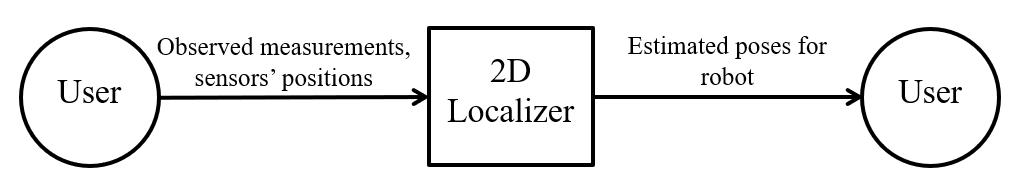
\includegraphics[width=0.6\textwidth]{SystemContextFigure.png}
\caption{System Context}
\label{Fig_SystemContext} 
\end{center}
\end{figure}
\begin{itemize}
\item User Responsibilities:
\begin{itemize}
\item Provide inputs including the coordinates of each environmental sensor and the measurements taken from them.
\item Evaluate the inputs to ensure all are their respective types
\end{itemize}
\item \progname{} Responsibilities:
\begin{itemize} 
\item Detect data type mismatch, such as a string of characters instead of a
  floating point number
\item Estimate the position and orientation of the robot
\end{itemize}
\end{itemize}

\subsection{User Characteristics}\label{SecUserCharacteristics}

The end user of 2D Localizer should have some familiarity with types of range sensors along with how to read and collect their data. They should also have basic experience with programming.

\subsection{System Constraints}

There are no system constraints.

\section{Specific System Description}

This section first presents the problem description, which gives a high-level
view of the problem to be solved.  This is followed by the solution characteristics
specification, which presents the assumptions, theories, definitions and finally
the instance models.

\subsection{Problem Description}\label{Sec_pd}

2D Localizer is intended to help keep track of mobile robots while carrying out their tasks.

\subsubsection{Terminology and  Definitions}

This subsection provides a list of terms that are used in the subsequent
sections and their meaning, with the purpose of reducing ambiguity and making it
easier to correctly understand the requirements:

\begin{itemize}

\item \textbf{Pose:} Position and orientation of the robot.
\item \textbf{Localization}: Determining where an object is with respect to its environment.
\item \textbf{Fiducial Markers}: Markers placed around the environment for the robot to determine its location.
\item \textbf{Beacon}: A range sensor

\end{itemize}

\subsubsection{Physical System Description}\label{sec_phySystDescrip}

\plt{The purpose of this section is to clearly and unambiguously state the
  physical system that is to be modelled. Effective problem solving requires a
  logical and organized approach. The statements on the physical system to be
  studied should cover enough information to solve the problem. The physical
  description involves element identification, where elements are defined as
  independent and separable items of the physical system. Some example elements
  include acceleration due to gravity, the mass of an object, and the size and
  shape of an object. Each element should be identified and labelled, with their
  interesting properties specified clearly. The physical description can also
  include interactions of the elements, such as the following: i) the
  interactions between the elements and their physical environment; ii) the
  interactions between elements; and, iii) the initial or boundary conditions.}

\plt{The elements of the physical system do not have to correspond to an actual
physical entity.  They can be conceptual.  This is particularly important when
the documentation is for a numerical method. }

The physical system of \progname{}, as shown in Figure~?,
includes the following elements:

\begin{itemize}

\item[PS1:] 

\item[PS2:] ...

\end{itemize}

\plt{A figure here makes sense for most SRS documents}

% \begin{figure}[h!]
% \begin{center}
% %\rotatebox{-90}
% {
%  \includegraphics[width=0.5\textwidth]{<FigureName>}
% }
% \caption{\label{<Label>} <Caption>}
% \end{center}
% \end{figure}

\subsubsection{Goal Statements}

\noindent Given the imported 2D map, coordinates of all sensors and fiducial markers in the environment, and the noisy measurements of the sensors, the goal statements are:

\begin{itemize}

\item[GS\refstepcounter{goalnum}1 \label{GS1}:] Calculate the estimated pose (position and orientation) and error of the robot throughout its trajectory from both sensors (environment and robot).
\item[GS\refstepcounter{goalnum}2 \label{GS2}:] Display a visual representation of the robot traversing the 2-D map with the sensors placed.

\end{itemize}

\subsection{Solution Characteristics Specification}

\plt{This section specifies the information in the solution domain of the system
  to be developed. This section is intended to express what is required in
  such a way that analysts and stakeholders get a clear picture, and the
  latter will accept it. The purpose of this section is to reduce the problem
  into one expressed in mathematical terms. Mathematical expertise is used to
  extract the essentials from the underlying physical description of the
  problem, and to collect and substantiate all physical data pertinent to the
  problem.}

\plt{This section presents the solution characteristics by successively refining
  models.  It starts with the abstract/general Theoretical Models (TMs) and
  refines them to the concrete/specific Instance Models (IMs).  If necessary
  there are intermediate refinements to General Definitions (GDs).  All of these
  refinements can potentially use Assumptions (A) and Data Definitions (DD).
  TMs are refined to create new models, that are called GMs or IMs. DDs are not
  refined; they are just used. GDs and IMs are derived, or refined, from other
  models. DDs are not derived; they are just given. TMs are also just given, but
  they are refined, not used.  If a potential DD includes a derivation, then
  that means it is refining other models, which would make it a GD or an IM.}

\plt{The above makes a distinction between ``refined'' and ``used.'' A model is
  refined to another model if it is changed by the refinement. When we change a
  general 3D equation to a 2D equation, we are making a refinement, by applying
  the assumption that the third dimension does not matter. If we use a
  definition, like the definition of density, we aren't refining, or changing
  that definition, we are just using it.}

\plt{The same information can be a TM in one problem and a DD in another.  It is
  about how the information is used.  In one problem the definition of
  acceleration can be a TM, in another it would be a DD.}

\plt{There is repetition between the information given in the different chunks
  (TM, GDs etc) with other information in the document.  For instance, the
  meaning of the symbols, the units etc are repeated.  This is so that the
  chunks can stand on their own when being read by a reviewer/user.  It also
  facilitates reuse of the models in a different context.}

\noindent \plt{The relationships between the parts of the document are show in
  the following figure.  In this diagram ``may ref'' has the same role as
  ``uses'' above.  The figure adds ``Likely Changes,'' which are able to
  reference (use) Assumptions.}

\begin{figure}[H]
  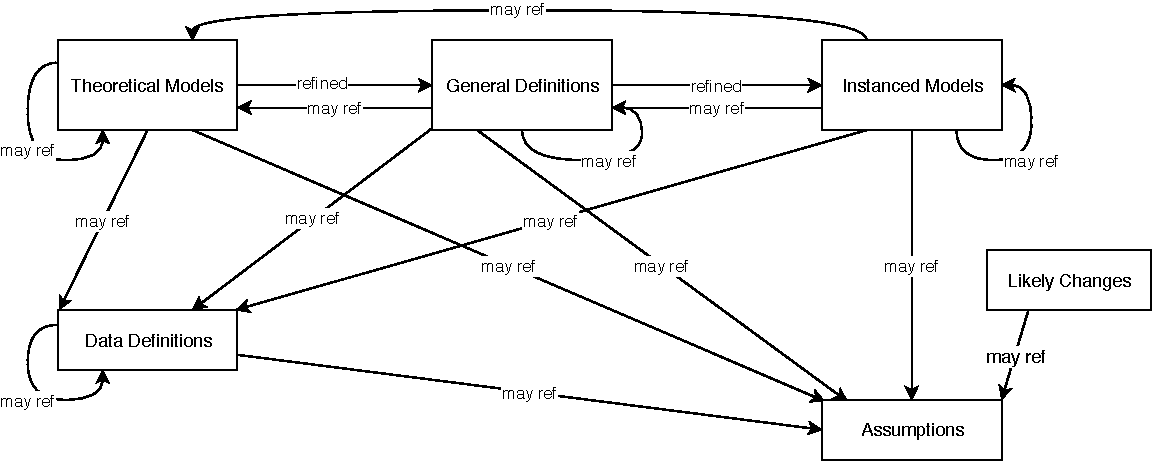
\includegraphics[scale=0.9]{RelationsBetweenTM_GD_IM_DD_A.pdf}
\end{figure}

The instance models that govern \progname{} are presented in
Subsection~\ref{sec_instance}.  The information to understand the meaning of the
instance models and their derivation is also presented, so that the instance
models can be verified.

\subsubsection{Types}

\plt{This section is optional. Defining types can make the document easier to
understand.}

\subsubsection{Scope Decisions}

\plt{This section is optional.}
\subsubsection{Modelling Decisions}

\plt{This section is optional.}

\subsubsection{Assumptions}\label{sec_assumpt}


This section simplifies the original problem and helps in developing the
theoretical model by filling in the missing information for the physical system.
The numbers given in the square brackets refer to the theoretical model [TM],
general definition [GD], data definition [DD], instance model [IM], or likely
change [LC], in which the respective assumption is used.

\begin{itemize}

\item[A\refstepcounter{assumpnum}1 \label{A_sensors}:]Robot uses camera sensors while the environment uses beacons and fiducial markers
\item[A\refstepcounter{assumpnum}2 \label{A_controlled}:]Localizer is used in a controlled environment (i.e., indoors)
\item[A\refstepcounter{assumpnum}1 \label{A_indep}:]Each sensor has independent measurements
\item[A\refstepcounter{assumpnum}1 \label{A_noise}:]Sensor noise is zero-mean Gaussian


\end{itemize}

\subsubsection{Theoretical Models}\label{sec_theoretical}

\plt{Theoretical models are sets of abstract mathematical equations or axioms
  for solving the problem described in Section ``Physical System Description''
  (Section~\ref{sec_phySystDescrip}). Examples of theoretical models are
  physical laws, constitutive equations, relevant conversion factors, etc.}

\plt{Optionally the theory section could be divided into subsections to provide
more structure and improve understandability and reusability.  Potential
subsections include the following: Context theories, background theories, helper
theories, generic theories, problem specific theories, final theories and
rationale theories.}

This section focuses on the general equations and laws that \progname{} is based
on.  \plt{Modify the examples below for your problem, and add additional models
  as appropriate.}

~\newline
%TM 1
\noindent
\deftheory
% #2 refname of theory
{TM:NRM}
% #3 label
{Noisy Range Measurement}
% #4 equation
{
  $g_j(x) = \lVert \mathbf{x_i} - \mathbf{a_j}\rVert + \eta_j$ 
}
% #5 description
{

The equation above gives the noisy range measurement $g_j$ (\si\metre) of the beacons placed in the environment (\aref{A_sensors}) where $\mathbf{x_i}$ is the position of the robot (\si\metre), $\mathbf{a_j}$ is the position of the jth beacon placed (\si\metre), and $\eta_j$ is the noise from the jth beacon (\si\metre) (\aref{A_noise}).
}
% #6 Notes
{
This measurement does not calculate the orientation.
}
% #7 Source
{
  \url{http://www.efunda.com/formulae/heat_transfer/conduction/overview_cond.cfm}
}
% #8 Referenced by
{
  \dref{ROCT}
}
% #9 Preconditions
{
None
}
% #1 derivation - not applicable by default
{}

~\newline

% TM2
\noindent
\deftheory
% #2 refname of theory
{TM:MLE}
% #3 label
{Maximum Likelihood Estimation}
% #4 equation
{
  $\widehat{x} = \arg\min p(\tilde{D}\vert x)$
}
% #5 description
{
  This equation gives the MLE which estimates the best position $\widehat{x}$ (\si\metre) to align based on the range measurements given. 
}
% #6 Notes
{
None.
}
% #7 Source
{
  \url{http://www.efunda.com/formulae/heat_transfer/conduction/overview_cond.cfm}
}
% #8 Referenced by
{
  \dref{ROCT}
}
% #9 Preconditions
{
None
}
% #1 derivation - not applicable by default
{}

%TM3
~\newline

\noindent
\deftheory
% #2 refname of theory
{TM:CF}
% #3 label
{Cost Function}
% #4 equation
{
  $C(x) = \sum_{j=1}^{N} \frac{1}{\sigma_j^2} \left(\tilde{d_j} - \lVert \mathbf{x_i} - \mathbf{a_j}\rVert \right)^2$
}
% #5 description
{
  The above equation gives the conservation of energy for transient heat transfer in a material
  of specific heat capacity $C$ (\si{\joule\per\kilogram\per\celsius}) and density $\rho$ 
  (\si{\kilogram\per\cubic\metre}), where $\bf q$ is the thermal flux vector (\si{\watt\per\square\metre}),
  $g$ is the volumetric heat generation
  (\si{\watt\per\cubic\metre}), $T$ is the temperature
  (\si{\celsius}),  $t$ is time (\si{\second}), and $\nabla$ is
  the gradient operator.  For this equation to apply, other forms
  of energy, such as mechanical energy, are assumed to be negligible in the
  system (\aref{A_OnlyThermalEnergy}).  In general, the material properties ($\rho$ and $C$) depend on temperature.
}
% #6 Notes
{
None.
}
% #7 Source
{
  \url{http://www.efunda.com/formulae/heat_transfer/conduction/overview_cond.cfm}
}
% #8 Referenced by
{
  \dref{ROCT}
}
% #9 Preconditions
{
None
}
% #1 derivation - not applicable by default
{}

%TM4
~\newline

\noindent
\deftheory
% #2 refname of theory
{TM:FIM}
% #3 label
{Fisher Information Matrix}
% #4 equation
{
  $\mathbf{I_j} \cong \frac{1}{\sigma_j^2} \left(\frac{\widehat{x}-a_j}{\lVert \widehat{x}-a_j \rVert} \right)\left(\frac{\widehat{x}-a_j}{\lVert \widehat{x}-a_j \rVert}\right)^T$
}
% #5 description
{
  The above equation gives the conservation of energy for transient heat transfer in a material
  of specific heat capacity $C$ (\si{\joule\per\kilogram\per\celsius}) and density $\rho$ 
  (\si{\kilogram\per\cubic\metre}), where $\bf q$ is the thermal flux vector (\si{\watt\per\square\metre}),
  $g$ is the volumetric heat generation
  (\si{\watt\per\cubic\metre}), $T$ is the temperature
  (\si{\celsius}),  $t$ is time (\si{\second}), and $\nabla$ is
  the gradient operator.  For this equation to apply, other forms
  of energy, such as mechanical energy, are assumed to be negligible in the
  system (\aref{A_OnlyThermalEnergy}).  In general, the material properties ($\rho$ and $C$) depend on temperature.
}
% #6 Notes
{
None.
}
% #7 Source
{
  \url{http://www.efunda.com/formulae/heat_transfer/conduction/overview_cond.cfm}
}
% #8 Referenced by
{
  \dref{ROCT}
}
% #9 Preconditions
{
None
}
% #1 derivation - not applicable by default
{}

%TM5
~\newline

\noindent
\deftheory
% #2 refname of theory
{TM:CRLB}
% #3 label
{Cram\'{e}r-Rao Lower Bound}
% #4 equation
{
  $Var( \hat{\theta}) \geq \frac{1}{I(\theta)}$
}
% #5 description
{
  The above equation gives the conservation of energy for transient heat transfer in a material
  of specific heat capacity $C$ (\si{\joule\per\kilogram\per\celsius}) and density $\rho$ 
  (\si{\kilogram\per\cubic\metre}), where $\bf q$ is the thermal flux vector (\si{\watt\per\square\metre}),
  $g$ is the volumetric heat generation
  (\si{\watt\per\cubic\metre}), $T$ is the temperature
  (\si{\celsius}),  $t$ is time (\si{\second}), and $\nabla$ is
  the gradient operator.  For this equation to apply, other forms
  of energy, such as mechanical energy, are assumed to be negligible in the
  system (\aref{A_OnlyThermalEnergy}).  In general, the material properties ($\rho$ and $C$) depend on temperature.
}
% #6 Notes
{
None.
}
% #7 Source
{
  \url{http://www.efunda.com/formulae/heat_transfer/conduction/overview_cond.cfm}
}
% #8 Referenced by
{
  \dref{ROCT}
}
% #9 Preconditions
{
None
}
% #1 derivation - not applicable by default
{}

%TM6
~\newline

\noindent
\deftheory
% #2 refname of theory
{TM:SE2}
% #3 label
{SE(2) Transformation}
% #4 equation
{
  $T_{robot} =  
    \begin{bmatrix}
      R(\theta) & t \\
      0 & 1\\
    \end{bmatrix}
     $
}
% #5 description
{
  The above equation gives the conservation of energy for transient heat transfer in a material
  of specific heat capacity $C$ (\si{\joule\per\kilogram\per\celsius}) and density $\rho$ 
  (\si{\kilogram\per\cubic\metre}), where $\bf q$ is the thermal flux vector (\si{\watt\per\square\metre}),
  $g$ is the volumetric heat generation
  (\si{\watt\per\cubic\metre}), $T$ is the temperature
  (\si{\celsius}),  $t$ is time (\si{\second}), and $\nabla$ is
  the gradient operator.  For this equation to apply, other forms
  of energy, such as mechanical energy, are assumed to be negligible in the
  system (\aref{A_OnlyThermalEnergy}).  In general, the material properties ($\rho$ and $C$) depend on temperature.
}
% #6 Notes
{
None.
}
% #7 Source
{
  \url{http://www.efunda.com/formulae/heat_transfer/conduction/overview_cond.cfm}
}
% #8 Referenced by
{
  \dref{ROCT}
}
% #9 Preconditions
{
None
}
% #1 derivation - not applicable by default
{}

\plt{``Ref.\ By'' is used repeatedly with the different types of information.
  This stands for Referenced By.  It means that the models, definitions and
  assumptions listed reference the current model, definition or assumption.
  This information is given for traceability.  Ref. By provides a pointer in the
  opposite direction to what we commonly do.  You still need to have a reference
  in the other direction pointing to the current model, definition or
  assumption.  As an example, if TM1 is referenced by GD2, that means that GD2 will
  explicitly include a reference to TM1.}

~\newline

\subsubsection{General Definitions}\label{sec_gendef}

\plt{General Definitions (GDs) are a refinement of one or more TMs, and/or of
  other GDs.  The GDs are less abstract than the TMs.  Generally the reduction
  in abstraction is possible through invoking (using/referencing) Assumptions.
  For instance, the TM could be Newton's Law of Cooling stated abstracting.  The
  GD could take the general law and apply it to get a 1D equation.}

This section collects the laws and equations that will be used in building the
instance models.

\plt{Some projects may not have any content for this section, but the section
  heading should be kept.}  \plt{Modify the examples below for your problem, and
  add additional definitions as appropriate.}

~\newline

\noindent
\begin{minipage}{\textwidth}
\renewcommand*{\arraystretch}{1.5}
\begin{tabular}{| p{\colAwidth} | p{\colBwidth}|}
\hline
\rowcolor[gray]{0.9}
Number& GD\refstepcounter{defnum}\thedefnum \label{NL}\\
\hline
Label &\bf Newton's law of cooling \\
\hline
% Units&$MLt^{-3}T^0$\\
% \hline
SI Units&\si{\watt\per\square\metre}\\
\hline
Equation&$ q(t) = h \Delta T(t)$  \\
\hline
Description &
Newton's law of cooling describes convective cooling from a surface.  The law is
stated as: the rate of heat loss from a body is proportional to the difference
in temperatures between the body and its surroundings.
\\
& $q(t)$ is the thermal flux (\si{\watt\per\square\metre}).\\
& $h$ is the heat transfer coefficient, assumed independent of $T$ (\aref{A_hcoeff})
	(\si{\watt\per\square\metre\per\celsius}).\\
&$\Delta T(t)$= $T(t) - T_{\text{env}}(t)$ is the time-dependent thermal gradient
between the environment and the object (\si{\celsius}).
\\
\hline
  Source & Citation here \\
  \hline
  Ref.\ By & \ddref{FluxCoil}, \ddref{FluxPCM}\\
  \hline
\end{tabular}
\end{minipage}\\

\subsubsection*{Detailed derivation of simplified rate of change of temperature}

\plt{This may be necessary when the necessary information does not fit in the
  description field.}
\plt{Derivations are important for justifying a given GD.  You want it to be
  clear where the equation came from.}

\subsubsection{Data Definitions}\label{sec_datadef}

\plt{The Data Definitions are definitions of symbols and equations that are
  given for the problem.  They are not derived; they are simply used by other
  models.  For instance, if a problem depends on density, there may be a data
  definition for the equation defining density.  The DDs are given information
  that you can use in your other modules.}

\plt{All Data Definitions should be used (referenced) by at least one other
  model.}

This section collects and defines all the data needed to build the instance
models. The dimension of each quantity is also given.  \plt{Modify the examples
  below for your problem, and add additional definitions as appropriate.}

~\newline

\noindent
\begin{minipage}{\textwidth}
\renewcommand*{\arraystretch}{1.5}
\begin{tabular}{| p{\colAwidth} | p{\colBwidth}|}
\hline
\rowcolor[gray]{0.9}
Number& DD\refstepcounter{datadefnum}\thedatadefnum\label{Joint_Like}\\
\hline
Label& \bf Joint Likelihood Function\\
\hline
Symbol &$p_j( \tilde{D}\vert x)$\\
\hline
% Units& $Mt^{-3}$\\
% \hline
  SI Units & \si{\watt\per\square\metre}\\
  \hline
  Equation&$q_C(t) = h_C (T_C - T_W(t))$, over area $A_C$\\
  \hline
  Description & 
                $T_C$ is the temperature of the coil (\si{\celsius}).  $T_W$ is the temperature of the water (\si{\celsius}).  
                The heat flux out of the coil, $q_C$ (\si{\watt\per\square\metre}), is found by
                assuming that Newton's Law 
                of Cooling applies (\aref{A_Newt_coil}).  This law (\dref{NL}) is used on the surface of
                the coil, which has area $A_C$ (\si{\square\metre}) and heat 
                transfer coefficient $h_C$
                (\si{\watt\per\square\metre\per\celsius}).  This equation
                assumes that the temperature of the coil is constant over time (\aref{A_tcoil}) and that it does not vary along the length
                of the coil (\aref{A_tlcoil}).
  \\
  \hline
  Sources& Citation here \\
  \hline
  Ref.\ By & \hyperref[TM:MLE]{TM:MLE}\\
  \hline
\end{tabular}
\end{minipage}\\

\noindent
\begin{minipage}{\textwidth}
\renewcommand*{\arraystretch}{1.5}
\begin{tabular}{| p{\colAwidth} | p{\colBwidth}|}
\hline
\rowcolor[gray]{0.9}
Number& DD\refstepcounter{datadefnum}\thedatadefnum\label{Likelihood}\\
\hline
Label& \bf Likelihood Function\\
\hline
Symbol &$p_j( \tilde{d_j}\vert x)$\\
\hline
% Units& $Mt^{-3}$\\
% \hline
  SI Units & \si{\watt\per\square\metre}\\
  \hline
  Equation&$q_C(t) = h_C (T_C - T_W(t))$, over area $A_C$\\
  \hline
  Description & 
                $T_C$ is the temperature of the coil (\si{\celsius}).  $T_W$ is the temperature of the water (\si{\celsius}).  
                The heat flux out of the coil, $q_C$ (\si{\watt\per\square\metre}), is found by
                assuming that Newton's Law 
                of Cooling applies (\aref{A_Newt_coil}).  This law (\dref{NL}) is used on the surface of
                the coil, which has area $A_C$ (\si{\square\metre}) and heat 
                transfer coefficient $h_C$
                (\si{\watt\per\square\metre\per\celsius}).  This equation
                assumes that the temperature of the coil is constant over time (\aref{A_tcoil}) and that it does not vary along the length
                of the coil (\aref{A_tlcoil}).
  \\
  \hline
  Sources& Citation here \\
  \hline
  Ref.\ By & \hyperref[TM:MLE]{TM:MLE}\\
  \hline
\end{tabular}
\end{minipage}\\

\subsubsection{Data Types}\label{sec_datatypes}

\plt{This section is optional.  In many scientific computing programs it isn't
  necessary, since the inputs and outpus are straightforward types, like reals,
  integers, and sequences of reals and integers.  However, for some problems it
  is very helpful to capture the type information.}

\plt{The data types are not derived; they are simply stated and used by other
  models.}

\plt{All data types must be used by at least one of the models.}

\plt{For the mathematical notation for expressing types, the recommendation is
  to use the notation of~\citet{HoffmanAndStrooper1995}.}

This section collects and defines all the data types needed to document the
models. \plt{Modify the examples below for your problem, and add additional
  definitions as appropriate.}

~\newline

\noindent
\begin{minipage}{\textwidth}
\renewcommand*{\arraystretch}{1.5}
\begin{tabular}{| p{\colAwidth} | p{\colBwidth}|}
  \hline
  \rowcolor[gray]{0.9}
  Type Name & Name for Type\\
  \hline
  Type Def & mathematical definition of the type\\
  \hline
  Description & description here
  \\
  \hline
  Sources & Citation here, if the type is borrowed from another source\\
  \hline
\end{tabular}
\end{minipage}\\

\subsubsection{Instance Models} \label{sec_instance}    

\plt{The motivation for this section is to reduce the problem defined in
  ``Physical System Description'' (Section~\ref{sec_phySystDescrip}) to one
  expressed in mathematical terms. The IMs are built by refining the TMs and/or
  GDs.  This section should remain abstract.  The SRS should specify the
  requirements without considering the implementation.}

This section transforms the problem defined in Section~\ref{Sec_pd} into 
one which is expressed in mathematical terms. It uses concrete symbols defined 
in Section~\ref{sec_datadef} to replace the abstract symbols in the models 
identified in Sections~\ref{sec_theoretical} and~\ref{sec_gendef}.

The goals \plt{reference your goals} are solved by \plt{reference your instance
  models}.  \plt{other details, with cross-references where appropriate.}
\plt{Modify the examples below for your problem, and add additional models as
  appropriate.}

~\newline

%Instance Model 1

\noindent
\begin{minipage}{\textwidth}
\renewcommand*{\arraystretch}{1.5}
\begin{tabular}{| p{\colAwidth} | p{\colBwidth}|}
  \hline
  \rowcolor[gray]{0.9}
  Number& IM\refstepcounter{instnum}\theinstnum \label{ewat}\\
  \hline
  Label& \bf Energy balance on water to find $T_W$\\
  \hline
  Input&$m_W$, $C_W$, $h_C$, $A_C$, $h_P$, $A_P$, $t_\text{final}$, $T_C$, 
  $T_\text{init}$, $T_P(t)$ from \iref{epcm}\\
  & The input is constrained so that $T_\text{init} \leq T_C$ (\aref{A_charge})\\
  \hline
  Output&$T_W(t)$, $0\leq t \leq t_\text{final}$, such that\\
  &$\frac{dT_W}{dt} = \frac{1}{\tau_W}[(T_C - T_W(t)) + {\eta}(T_P(t) - T_W(t))]$,\\
  &$T_W(0) = T_P(0) = T_\text{init}$ (\aref{A_InitTemp}) and $T_P(t)$ from \iref{epcm} \\
  \hline
  Description&$T_W$ is the water temperature (\si{\celsius}).\\
  &$T_P$ is the PCM temperature (\si{\celsius}).\\
  &$T_C$ is the coil temperature (\si{\celsius}).\\
  &$\tau_W = \frac{m_W C_W}{h_C A_C}$ is a constant (\si{\second}).\\
  &$\eta = \frac{h_P A_P}{h_C A_C}$ is a constant (dimensionless).\\
  & The above equation applies as long as the water is in liquid form,
  $0<T_W<100^o\text{C}$, where $0^o\text{C}$ and $100^o\text{C}$ are the melting
  and boiling points of water, respectively (\aref{A_OpRange}, \aref{A_Pressure}).
  \\
  \hline
  Sources& Citation here \\
  \hline
  Ref.\ By & \iref{epcm}\\
  \hline
\end{tabular}
\end{minipage}\\

%~\newline

\subsubsection*{Derivation of ...}

\plt{The derivation shows how the IM is derived from the TMs/GDs.  In cases
  where the derivation cannot be described under the Description field, it will
  be necessary to include this subsection.}

\subsubsection{Input Data Constraints} \label{sec_DataConstraints}    

Table~\ref{TblInputVar} shows the data constraints on the input output
variables.  The column for physical constraints gives the physical limitations
on the range of values that can be taken by the variable.  The column for
software constraints restricts the range of inputs to reasonable values.  The
software constraints will be helpful in the design stage for picking suitable
algorithms.  The constraints are conservative, to give the user of the model the
flexibility to experiment with unusual situations.  The column of typical values
is intended to provide a feel for a common scenario.  The uncertainty column
provides an estimate of the confidence with which the physical quantities can be
measured.  This information would be part of the input if one were performing an
uncertainty quantification exercise.

The specification parameters in Table~\ref{TblInputVar} are listed in
Table~\ref{TblSpecParams}.

\begin{table}[!h]
  \caption{Input Variables} \label{TblInputVar}
  \renewcommand{\arraystretch}{1.2}
\noindent \begin{longtable*}{l l l l c} 
  \toprule
  \textbf{Var} & \textbf{Physical Constraints} & \textbf{Software Constraints} &
                             \textbf{Typical Value} & \textbf{Uncertainty}\\
  \midrule 
  $L$ & $L > 0$ & $L_{\text{min}} \leq L \leq L_{\text{max}}$ & 1.5 \si[per-mode=symbol] {\metre} & 10\%
  \\
  \bottomrule
\end{longtable*}
\end{table}

\noindent 
\begin{description}
\item[(*)] \plt{you might need to add some notes or clarifications}
\end{description}

\begin{table}[!h]
\caption{Specification Parameter Values} \label{TblSpecParams}
\renewcommand{\arraystretch}{1.2}
\noindent \begin{longtable*}{l l} 
  \toprule
  \textbf{Var} & \textbf{Value} \\
  \midrule 
  $L_\text{min}$ & 0.1 \si{\metre}\\
  \bottomrule
\end{longtable*}
\end{table}

\subsubsection{Properties of a Correct Solution} \label{sec_CorrectSolution}

\noindent
A correct solution must exhibit \plt{fill in the details}.  \plt{These
  properties are in addition to the stated requirements.  There is no need to
  repeat the requirements here.  These additional properties may not exist for
  every problem.  Examples include conservation laws (like conservation of
  energy or mass) and known constraints on outputs, which are usually summarized
  in tabular form.  A sample table is shown in Table~\ref{TblOutputVar}}

\begin{table}[!h]
\caption{Output Variables}\label{TblOutputVar}
\renewcommand{\arraystretch}{1.2}
\noindent \begin{longtable*}{l l} 
  \toprule
  \textbf{Var} & \textbf{Physical Constraints} \\
  \midrule 
  $T_W$ & $T_\text{init} \leq T_W \leq T_C$ (by~\aref{A_charge})
  \\
  \bottomrule
\end{longtable*}
\end{table}

\plt{This section is not for test cases or techniques for verification and
  validation.  Those topics will be addressed in the Verification and Validation
  plan.}

\section{Requirements}

\plt{The requirements refine the goal statement.  They will make heavy use of
  references to the instance models.}

This section provides the functional requirements, the business tasks that the
software is expected to complete, and the nonfunctional requirements, the
qualities that the software is expected to exhibit.

\subsection{Functional Requirements}

\noindent \begin{itemize}

\item[R\refstepcounter{reqnum}\thereqnum \label{R_Inputs}:] \plt{Requirements
    for the inputs that are supplied by the user.  This information has to be
    explicit.}

\item[R\refstepcounter{reqnum}\thereqnum \label{R_OutputInputs}:] \plt{It isn't
    always required, but often echoing the inputs as part of the output is a
    good idea.}

\item[R\refstepcounter{reqnum}\thereqnum \label{R_Calculate}:] \plt{Calculation
    related requirements.}

\item[R\refstepcounter{reqnum}\thereqnum \label{R_VerifyOutput}:]
  \plt{Verification related requirements.}

\item[R\refstepcounter{reqnum}\thereqnum \label{R_Output}:] \plt{Output related
    requirements.}

\end{itemize}

\plt{Every IM should map to at least one requirement, but not every requirement
  has to map to a corresponding IM.}

\subsection{Nonfunctional Requirements}

\plt{List your nonfunctional requirements.  You may consider using a fit
  criterion to make them verifiable.}
\plt{The goal is for the nonfunctional requirements to be unambiguous, abstract
  and verifiable.  This isn't easy to show succinctly, so a good strategy may be
to give a ``high level'' view of the requirement, but allow for the details to
be covered in the Verification and Validation document.}
\plt{An absolute requirement on a quality of the system is rarely needed.  For
  instance, an accuracy of 0.0101 \% is likely fine, even if the requirement is
  for 0.01 \% accuracy.  Therefore, the emphasis will often be more on
  describing now well the quality is achieved, through experimentation, and
  possibly theory, rather than meeting some bar that was defined a priori.}
\plt{You do not need an entry for correctness in your NFRs.  The purpose of the
  SRS is to record the requirements that need to be satisfied for correctness.
  Any statement of correctness would just be redundant. Rather than discuss
  correctness, you can characterize how far away from the correct (true)
  solution you are allowed to be.  This is discussed under accuracy.}

\noindent \begin{itemize}

\item[NFR\refstepcounter{nfrnum}\thenfrnum \label{NFR_Accuracy}:]
  \textbf{Accuracy} \plt{Characterize the accuracy by giving the context/use for
    the software.  Maybe something like, ``The accuracy of the computed
    solutions should meet the level needed for $<$engineering or scientific
    application$>$.  The level of accuracy achieved by \progname{} shall be
    described following the procedure given in Section~X of the Verification and
    Validation Plan.''  A link to the VnV plan would be a nice extra.}

\item[NFR\refstepcounter{nfrnum}\thenfrnum \label{NFR_Usability}:] \textbf{Usability}
  \plt{Characterize the usability by giving the context/use for the software.
    You should likely reference the user characteristics section.  The level of
    usability achieved by the software shall be described following the
    procedure given in Section~X of the Verification and Validation Plan.  A
    link to the VnV plan would be a nice extra.}

\item[NFR\refstepcounter{nfrnum}\thenfrnum \label{NFR_Maintainability}:]
  \textbf{Maintainability} \plt{The effort required to make any of the likely
    changes listed for \progname{} should be less than FRACTION of the original
    development time.  FRACTION is then a symbolic constant that can be defined
    at the end of the report.}

\item[NFR\refstepcounter{nfrnum}\thenfrnum \label{NFR_Portability}:]
  \textbf{Portability} \plt{This NFR is easier to write than the others.  The
    systems that \progname{} should run on should be listed here.  When possible
    the specific versions of the potential operating environments should be
    given.  To make the NFR verifiable a statement could be made that the tests
    from a given section of the VnV plan can be successfully run on all of the
    possible operating environments.}

\item Other NFRs that might be discussed include verifiability,
  understandability and reusability.

\end{itemize}

\subsection{Rationale}

\plt{Provide a rationale for the decisions made in the documentation.  Rationale
should be provided for scope decisions, modelling decisions, assumptions and
typical values.}

\section{Likely Changes}    

\noindent \begin{itemize}

\item[LC\refstepcounter{lcnum}\thelcnum\label{LC_meaningfulLabel1}:] \plt{Give
    the likely changes, with a reference to the related assumption (aref), as appropriate.}

\end{itemize}

\section{Unlikely Changes}    

\noindent \begin{itemize}

\item[LC\refstepcounter{lcnum}\thelcnum\label{LC_meaningfulLabel2}:] \plt{Give
    the unlikely changes.  The design can assume that the changes listed will
    not occur.}

\end{itemize}

\section{Traceability Matrices and Graphs}

The purpose of the traceability matrices is to provide easy references on what
has to be additionally modified if a certain component is changed.  Every time a
component is changed, the items in the column of that component that are marked
with an ``X'' may have to be modified as well.  Table~\ref{Table:trace} shows the
dependencies of theoretical models, general definitions, data definitions, and
instance models with each other. Table~\ref{Table:R_trace} shows the
dependencies of instance models, requirements, and data constraints on each
other. Table~\ref{Table:A_trace} shows the dependencies of theoretical models,
general definitions, data definitions, instance models, and likely changes on
the assumptions.

\plt{You will have to modify these tables for your problem.}

\plt{The traceability matrix is not generally symmetric.  If GD1 uses A1, that
  means that GD1's derivation or presentation requires invocation of A1.  A1
  does not use GD1.  A1 is ``used by'' GD1.}

\plt{The traceability matrix is challenging to maintain manually.  Please do
  your best.  In the future tools (like Drasil) will make this much easier.}

\afterpage{
\begin{landscape}
\begin{table}[h!]
\centering
\begin{tabular}{|c|c|c|c|c|c|c|c|c|c|c|c|c|c|c|c|c|c|c|c|}
\hline
	& \aref{A_OnlyThermalEnergy}& \aref{A_hcoeff}& \aref{A_mixed}& \aref{A_tpcm}& \aref{A_const_density}& \aref{A_const_C}& \aref{A_Newt_coil}& \aref{A_tcoil}& \aref{A_tlcoil}& \aref{A_Newt_pcm}& \aref{A_charge}& \aref{A_InitTemp}& \aref{A_OpRangePCM}& \aref{A_OpRange}& \aref{A_htank}& \aref{A_int_heat}& \aref{A_vpcm}& \aref{A_PCM_state}& \aref{A_Pressure} \\
\hline
\tref{T_COE}        & X& & & & & & & & & & & & & & & & & & \\ \hline
\tref{T_SHE}        & & & & & & & & & & & & & & & & & & & \\ \hline
\tref{T_LHE}        & & & & & & & & & & & & & & & & & & & \\ \hline
\dref{NL}           & & X& & & & & & & & & & & & & & & & & \\ \hline
\dref{ROCT}         & & & X& X& X& X& & & & & & & & & & & & & \\ \hline
\ddref{FluxCoil}    & & & & & & & X& X& X& & & & & & & & & & \\ \hline
\ddref{FluxPCM}     & & & X& X& & & & & & X& & & & & & & & & \\ \hline
\ddref{D_HOF}       & & & & & & & & & & & & & & & & & & & \\ \hline
\ddref{D_MF}        & & & & & & & & & & & & & & & & & & & \\ \hline
\iref{ewat}         & & & & & & & & & & & X& X& & X& X& X& & & X \\ \hline
\iref{epcm}         & & & & & & & & & & & & X& X& & & X& X& X& \\ \hline
\iref{I_HWAT}       & & & & & & & & & & & & & & X& & & & & X \\ \hline
\iref{I_HPCM}       & & & & & & & & & & & & & X& & & & & X & \\ \hline
\lcref{LC_tpcm}     & & & & X& & & & & & & & & & & & & & & \\ \hline
\lcref{LC_tcoil}    & & & & & & & & X& & & & & & & & & & & \\ \hline
\lcref{LC_tlcoil}   & & & & & & & & & X& & & & & & & & & & \\ \hline
\lcref{LC_charge}   & & & & & & & & & & & X& & & & & & & & \\ \hline
\lcref{LC_InitTemp} & & & & & & & & & & & & X& & & & & & & \\ \hline
\lcref{LC_htank}    & & & & & & & & & & & & & & & X& & & & \\
\hline
\end{tabular}
\caption{Traceability Matrix Showing the Connections Between Assumptions and Other Items}
\label{Table:A_trace}
\end{table}
\end{landscape}
}

\begin{table}[h!]
\centering
\begin{tabular}{|c|c|c|c|c|c|c|c|c|c|c|c|c|c|c|c|c|c|c|c|c|c|c|c|}
\hline        
	& \tref{T_COE}& \tref{T_SHE}& \tref{T_LHE}& \dref{NL}& \dref{ROCT} & \ddref{FluxCoil}& \ddref{FluxPCM} & \ddref{D_HOF}& \ddref{D_MF}& \iref{ewat}& \iref{epcm}& \iref{I_HWAT}& \iref{I_HPCM} \\
\hline
\tref{T_COE}     & & & & & & & & & & & & & \\ \hline
\tref{T_SHE}     & & & X& & & & & & & & & & \\ \hline
\tref{T_LHE}     & & & & & & & & & & & & & \\ \hline
\dref{NL}        & & & & & & & & & & & & & \\ \hline
\dref{ROCT}      & X& & & & & & & & & & & & \\ \hline
\ddref{FluxCoil} & & & & X& & & & & & & & & \\ \hline
\ddref{FluxPCM}  & & & & X& & & & & & & & & \\ \hline
\ddref{D_HOF}    & & & & & & & & & & & & & \\ \hline
\ddref{D_MF}     & & & & & & & & X& & & & & \\ \hline
\iref{ewat}      & & & & & X& X& X& & & & X& & \\ \hline
\iref{epcm}      & & & & & X& & X& & X& X& & & X \\ \hline
\iref{I_HWAT}    & & X& & & & & & & & & & & \\ \hline
\iref{I_HPCM}    & & X& X& & & & X& X& X& & X& & \\
\hline
\end{tabular}
\caption{Traceability Matrix Showing the Connections Between Items of Different Sections}
\label{Table:trace}
\end{table}

\begin{table}[h!]
\centering
\begin{tabular}{|c|c|c|c|c|c|c|c|}
\hline
	& \iref{ewat}& \iref{epcm}& \iref{I_HWAT}& \iref{I_HPCM}& \ref{sec_DataConstraints}& \rref{R_RawInputs}& \rref{R_MassInputs} \\
\hline
\iref{ewat}            & & X& & & & X& X \\ \hline
\iref{epcm}            & X& & & X& & X& X \\ \hline
\iref{I_HWAT}          & & & & & & X& X \\ \hline
\iref{I_HPCM}          & & X& & & & X& X \\ \hline
\rref{R_RawInputs}     & & & & & & & \\ \hline
\rref{R_MassInputs}    & & & & & & X& \\ \hline
\rref{R_CheckInputs}   & & & & & X& & \\ \hline
\rref{R_OutputInputs}  & X& X& & & & X& X \\ \hline
\rref{R_TempWater}     & X& & & & & & \\ \hline 
\rref{R_TempPCM}       & & X& & & & & \\ \hline
\rref{R_EnergyWater}   & & & X& & & & \\ \hline
\rref{R_EnergyPCM}     & & & & X& & & \\ \hline
\rref{R_VerifyOutput}  & & & X& X& & & \\ \hline
\rref{R_timeMeltBegin} & & X& & & & & \\ \hline
\rref{R_timeMeltEnd}   & & X& & & & & \\ 
\hline
\end{tabular}
\caption{Traceability Matrix Showing the Connections Between Requirements and Instance Models}
\label{Table:R_trace}
\end{table}

The purpose of the traceability graphs is also to provide easy references on
what has to be additionally modified if a certain component is changed.  The
arrows in the graphs represent dependencies. The component at the tail of an
arrow is depended on by the component at the head of that arrow. Therefore, if a
component is changed, the components that it points to should also be
changed. Figure~\ref{Fig_ATrace} shows the dependencies of theoretical models,
general definitions, data definitions, instance models, likely changes, and
assumptions on each other. Figure~\ref{Fig_RTrace} shows the dependencies of
instance models, requirements, and data constraints on each other.

% \begin{figure}[h!]
% 	\begin{center}
% 		%\rotatebox{-90}
% 		{
% 			\includegraphics[width=\textwidth]{ATrace.png}
% 		}
% 		\caption{\label{Fig_ATrace} Traceability Matrix Showing the Connections Between Items of Different Sections}
% 	\end{center}
% \end{figure}


% \begin{figure}[h!]
% 	\begin{center}
% 		%\rotatebox{-90}
% 		{
% 			\includegraphics[width=0.7\textwidth]{RTrace.png}
% 		}
% 		\caption{\label{Fig_RTrace} Traceability Matrix Showing the Connections Between Requirements, Instance Models, and Data Constraints}
% 	\end{center}
% \end{figure}

\section{Development Plan}

\plt{This section is optional.  It is used to explain the plan for developing
  the software.  In particular, this section gives a list of the order in which
  the requirements will be implemented.  In the context of a course  this is
  where you can indicate which requirements will be implemented as part of the
  course, and which will be ``faked'' as future work.  This section can be
  organized as a prioritized list of requirements, or it could should the
  requirements that will be implemented for ``phase 1'', ``phase 2'', etc.}

\section{Values of Auxiliary Constants}

\plt{Show the values of the symbolic parameters introduced in the report.}

\plt{The definition of the requirements will likely call for SYMBOLIC\_CONSTANTS.
Their values are defined in this section for easy maintenance.}

\plt{The value of FRACTION, for the Maintainability NFR would be given here.}

\newpage

\bibliographystyle {plainnat}
\bibliography {../../refs/References}

\newpage

\noindent \plt{The following is not part of the template, just some things to consider
  when filing in the template.}

\noindent \plt{Grammar, flow and \LaTeX advice:
\begin{itemize}
\item For Mac users \texttt{*.DS\_Store} should be in \texttt{.gitignore}
\item \LaTeX{} and formatting rules
\begin{itemize}
\item Variables are italic, everything else not, includes subscripts (link to
  document)
\begin{itemize}
\item \href{https://physics.nist.gov/cuu/pdf/typefaces.pdf}{Conventions}
\item Watch out for implied multiplication
\end{itemize}
\item Use BibTeX
\item Use cross-referencing
\end{itemize}
\item Grammar and writing rules
\begin{itemize}
\item Acronyms expanded on first usage (not just in table of acronyms)
\item ``In order to'' should be ``to''
\end{itemize}
\end{itemize}}

\noindent \plt{Advice on using the template:
\begin{itemize}
\item Difference between physical and software constraints
\item Properties of a correct solution means \emph{additional} properties, not
  a restating of the requirements (may be ``not applicable'' for your problem).
  If you have a table of output constraints, then these are properties of a
  correct solution.
\item Assumptions have to be invoked somewhere
\item ``Referenced by'' implies that there is an explicit reference
\item Think of traceability matrix, list of assumption invocations and list of
  reference by fields as automatically generatable
\item If you say the format of the output (plot, table etc), then your
  requirement could be more abstract
\end{itemize}
}

\newpage{} 

\end{document}